\documentclass[a4paper]{article}

%% Language and font encodings
\usepackage[english]{babel}
\usepackage[utf8x]{inputenc}
\usepackage[T1]{fontenc}

%% Sets page size and margins
\usepackage[a4paper,top=4cm,bottom=4cm,left=4cm,right=4cm,marginparwidth=1.75cm]{geometry}

%% Useful packages
\usepackage{amsmath}
\usepackage{url}
\usepackage{graphicx}
\usepackage[colorinlistoftodos]{todonotes}
\usepackage[colorlinks=true, allcolors=blue]{hyperref}
\usepackage[font={small,it}]{caption}
\usepackage{amsmath}
\usepackage{graphicx}
\usepackage{tikz}
\usepackage{pgfplots}
\usepackage{pgfplotstable}
\usepackage{multirow}
\usepackage{comment}
\usepackage{algorithm2e}
\usepackage{algorithmic}
\usepackage{titlesec}
\usepackage{caption}
\usepackage{subcaption}
\pgfdeclarelayer{f}
\pgfsetlayers{main,f}

\setcounter{secnumdepth}{4}

\titleformat{\paragraph}
{\normalfont\normalsize\bfseries}{\theparagraph}{1em}{}
\titlespacing*{\paragraph}
{0pt}{3.25ex plus 1ex minus .2ex}{1.5ex plus .2ex}


\title{Evaluating the use of ICN for Internet of things}
\author{Johan Carlquist}

\begin{document}
\maketitle
\newpage
\begin{abstract}
% Your abstract.
% \begin{itemize}
% 	\item Written last
% 	\item Sell your idea!\\
% 	make the reader wnat to stay with you
% 	\item Single paragraph, 100-200 words
% 	\item for parths/sentences
% 	\begin{enumerate}
% 		\item What is your problem
% 		The market of IoT devices continues to grow at a rapid speed as well as constrained wireless sensor networks.
% 		Today, the main network paradigm is \textit{host centric} where a users have to specify which host they want to %receive their data from. Information-centric networking is a new paradigm for the future internet, which is based %on \textit{named data} instead of \textit{named hosts}. With ICN, a user sends a request for a perticular data on %the network, any router or server containing the data will respond to the request.
%
%
%		\item How did you solve it
%	\end{enumerate}
%	By creating an algortihm that follow the interval of the sensor, one can acheive similar 
%	\begin{enumerate}
%		\item What are the results
%		\item Conclusions (what it means for the futrue)
% 	\end{enumerate}
% 	\item Make sure the abstract stands on its own!
% 	\end{itemize}
The market of IoT devices continues to grow at a rapid speed as well as constrained wireless sensor networks.
Today, the main network paradigm is \textit{host centric} where a users have to specify which host they want to receive their data from. Information-centric networking is a new paradigm for the future internet, which is based on \textit{named data} instead of \textit{named hosts}. With ICN, a user sends a request for a perticular data on the network, any router or server containing the data will respond to the request.

In order to achieve low latency between data creation and its consumption, as well as being able to follow the sequential production of data, an algorithm was created for these purposes during this thesis. This algorithm uses a `one-time subscription' approach to initiate a \textit{interest} message before the data has been created at the sensor.

The result of this algorithm shows that a consumer can retrieve the data with minimum latency from its creation by the sensor, without using a publish/subscribe system such as MQTT or similar. The study shows that it can handle larger variations of clock drift from the sensor. 
The performance evaluation carried out which analysed the Content Centric Network application on the sensor shows that the application has little impact on the overall round trip time in the network.

Based on the results, this thesis concluded that the ICN paradigm, together with a 'one-time subscription' model, can be a suitable option for communication within the IoT domain where consumers ask for sequentially produced data. 





\end{abstract}

\newpage
\section*{Populärvetenskaplig sammanfattning}
IoT kan vara en del av framtidens Internet, där datat förflyttas.
\newpage
\section*{Acknowledgement}

I would like to take this opportunity to sincerely thank my two supervisors, Bengt Ahlgren and Anders Lindgren from Research Institute of Sweden for their valuable support and input throughout the entire thesis project. Without their help and great knowledge, this project would not have succeeded.\\\\
I would also like to thank my mentor Edith Ngai for the feedback, discussions and relevent input of which made it possible to complete this thesis.\\\\
Furthermore, I would like to take the opportunity to thank Valtech Sweden for their support and help with computer equiment and more.\\\\
Last but not the least, I would like to thank Anna Rumetshofer who has helped with encouraging, read through and general advices regarding the writing part of the thesis.\\\\


%Lastly we would like to thank or mentor Justin Pearson for all feedback, dis- cussions and relevant input, without which this thesis would not have been completed.






\newpage

\tableofcontents
\newpage
%\listoffigures
%\newpage

\section{Introduction}
The main paradigm of networks today can be called  \textit{host centric} and most of our communication is defined as end-to-end between these hosts. It is predicted that in 2020 we reach around 50 billion Internet of Things (IoT) devices \cite{alanCarlton} and the usage of these devices often imply information centric usage patterns \cite{Ahlgren2012}.\todo{Hela introt lite väl kort...} \todo{Borde nämna ``named hosts'' här också.}
\\\\
Information-centric networking (ICN) is a communication paradigm for the future Internet that is based on \textit{named data} instead of \textit{named hosts}. The communication is defined through requesting and providing named data, decoupling senders from receivers. This could make it possible to integrate storage for caching within the network infrastructure \cite{Ahlgren2012} which could lead to improvements in the network as a whole.

\begin{itemize}
	\item Rewrite.
	\item Write this lastly.
\end{itemize}


%Recently there has been some investigation about the applicability and trade-offs of the ICN paradigm in the IoT/sensor domain \cite{surveyPaper2}. It will be interesting to investigate the mapping of IoT-sensor data directly to \textit{named data} in ICN and therefore use the network as an application-independent distribution for IoT data values. 

\subsection{Motivation}
\begin{itemize}
	\item Remove this and put it under introduction instead?
\end{itemize}

\subsection{Problem statement}
%The overal objective with this thesis is to make an experimental evaluation of the performance and applicability of using ICN in the IoT/sensor domain. The goal is to assess the feasibility and performance

The purpose of this thesis project is to evaluate the performance and feasibility of using the ICN paradigm in the IoT domain. The scenarios are normal usage patterns between devices including producing and consuming data continuously created in a periodic interval. By evaluating the performance of ICN components and the application as a whole, one can provide a comparision between such an application and a network reference \todo{vad menas med ref point och resterande del av meningen. // A} point. Ideally it should be possible \todo{Formulera om. // A} to divide and present the throughput, and how much delay time, spent operating under ICN. Therefore a part of the goal of this thesis project is to provide an in depth analysis of where most time is spent when using the ICN application. 

%Another goal of the performance is to investigate how well ICN can scale as the network increases in size, main focus is considered when several consumers want to access data that is provided by one producer.

ICN is by nature a pull paradigm where a consumer has to initiate a request of a particular data object in order to retrive it. This is in constrast to several IoT systems where the publish/subscribe approach is more common. An example of such a system is MQTT \cite{mqtt} where the producer sends the newly created data towards a broker, which then pushes the data to a user/consumer. By evaluating the feasibility, a major goal is to investigate if it is possible to achive similar outcome with ICN together with a onetime subscription model and if such a system would be stable. With the onetime subscription model, a consumer tries to pull the data from the producers by initiating a request just before the data has been created.



\subsection{Delimitations}
CCN will be the only ICN architecture covered in this thesis. Alternative implementations such as Psirp, Netinf among others, will not be covered at all.
Furthermore, this thesis will not develop any further functionallity on the current CCN implementation for Contiki-OS. The current implementaion is to be considered sufficient. Exceptions are made for functionallity regarding monitoring and measurement metrics that will have effect on the evaluation. Different cache strategies for the local storage at a CCN node and other functionallities that would be desirable, but not necessary, is considered out of the scope of this thesis. Furthermore, no aspect of power consumption will be taken into account for the thesis.


\subsection{Research methodology}
\todo{Behöver kompletteras med lite mer generell text om experimentell forskning.// B}
Currently there is a \todo{Berätta att ccn-lite är en lw impl av ccn, sen har yanqiu portat det till contiki.// a} CCN-lite implementation for the IoT light-weighted Contiki OS, the implementation was conducted by a former thesis worker Yanqiu Wu \cite{yanqui}. In this project, a qualitative and quantitative performance evaluation will be carried out through experimentation with this implementation. The sensor hardware used is the Texas Instruments SensorTag CC2650, which runs the CCN-lite implementation. \\\\
Since the thesis is based on experiments a large amount of measurements will be conducted. The methodology used will be \todo{Short cycels of what? // a}short cycles and small loops between each measurement. This iterative approach has the advantage that it can give answers to \todo{Formulera om, vad är det som menas? // a}questions that are not specifically asked and it can also be used to see changes over time. 
In order to make the testing intervals short and feasible, a lot of effort has been put into creating smart scripts that automate testing and representation of the data so it becomes visual to the tester. 
\\\\
Different software tools will be programmed to measure the desired performance metrics. 
In order to evaluate the performance, various types of measuring tools will be conducted. These tools has either a general or a specific purpose. A general purpose tool can for instance collect the measured data from the test, and make it representable for the user. Specific purpose tools on the other hand can be ones that measure the processing time on a sensor or measure the latency time. 

\subsection{Contributions}

This thesis contribute an experimental evaluation, with performance and feasibility aspects in focus, of using CCN on low power sensor hardware in a typical IoT enviroment.

There are several other contributions of this thesis project. One is improving the current CCN-lite application for Contiki-OS, mostly to make it more stable and reliable when run on low power sensor hardware. Another contribution is the development of a tool that calculates the roundtrip times for IPv6 devices to the CCN-lite project. Moreover, software enabling a consumer to retrieve data from the publisher through a one-time subscription model described in later parts.



Furthermore, several testing tools have been developed to make this thesis possible. Although a lot of time and effort has been consumed into creating these software implementations, the specific details concerning implementation will not be covered in this report. However, some higher abstractation regarding algorithms and logics will be presented.


\subsection{Related work}
%\begin{itemize}
%	\item MQTT - the most popular application layer protocol for IoT networks. Designed to be a lightweight communication protocol between machine devices. Although its popularity, it comes with shortages %such as TCP only, large overheads [Remove??]
%	\item ICN as a whole - Several studies describe the benefits when using ICN. A majority of them come from the academic work 
%							Several studies describe the benefits using ICN on a conceptual level, few studies show the real implementation regarding replacing the IP network -> there are exceptions.
%	\item IoT and ICN/CCN - Due to the high likelyness between IoT and ICN, several studies has shown that there can be benefits when using ICN in the IoT domain. 
%	\item CCN - CCN is one of the candidates available, 
%	\item Outline ideas as `onetime subscriptions' n others. 
%	\item Yanquie
%\end{itemize}

When Jacobson et al. publicated the paper \textit{Networking named content} in 2009 it sparked ideas of an alternative approach of communicating in contrast to current IP networking \cite{Jacobson2009}. They implemented a prototype which replaced IP with CCN in the network stack and proved that it could be a potential alternative for the future Internet.
Since then, several research papers have been published comparing different ICN alternatives and their potential benefits and trade-offs when implemented as a network service\cite{Ahlgren2012}. Studies prove that it could be a suitable replacement of current IP networking structures, but there is a need for more performance analysis and studies\cite{Ahlgren2012}\cite{Greek-ICN-networking-survey-2014}.

However, it was not until the last couple of years that the research community started to investigate the feasibility and applicability of using ICN in the IoT domain. Several studies, the majority being literature studies and theories, have been conducted recently or are currently ongoing. There only seem to be two implementation studies available to date.

In a concept study conducted by Ahlgren et al. \cite{Ahlgreniot}, they conclude that an advantage with ICN, the naming of data, is independent of the device that produces it. The decoupling between a publisher and subscriber of data could improve performance in lossy networks\todo{Behöver koppla named data till IoT-context - Namngivet sensordata}.Challenges reside in the naming of data that is produced periodically over time where a major issue is to retrieve the \textit{latest} value in that sequence. Potential solutions could be to implement a \textit{one-time subscription}, where the request is stored in the cache at the node until the data becomes available\cite{Ahlgreniot}. 

In another study provided by Amadeo et al. \cite{iotchop} argues ICN is by nature close to the IoT domain. They also conclude that there is a need of further investigations regarding if ICN should be implemented as an overlay of existing IP infrastructure, coexist with IP, or if it should be a replacement in the same manner as proposed in \cite{Jacobson2009}.

Baccelli et al. were first to implement a portation for CCN-lite to the IoT operating system RIOT \cite{icniotexpinwild}\cite{RIOT}. That project was the first trial of implementing ICN without any IP protocol. They compared their CCN-lite implemententation and a regular 6LowPAN/IPv6/RPL approach and saw that there were several advantages using ICN over IP. Although they identified several areas where further work needs to be done, they argue that ICN is applicable in the IoT domain.

Another implementation of CCN for IoT devices was a thesis project conducted by Yanqui Wu at SICS/KTH\cite{yanqui}. He ported the CCN-lite functionallity into another IoT operating system, Contiki-OS, and implemented the software as an middle-layer between the application- and the transport layer. Although some evaluation was done, there was no further investigation on how well CCN performs at the application layer. \\

%\begin{itemize}
%\item Either part of the introduction or after the body
%	\begin{itemize}
%		\item after the body is eaiser to explain.
%	\end{itemize}
%\item Credit is not like money
%	\begin{itemize}
%		\item Giving credit to someone else does not take it away from yours.
%		\item faling to give credit though.
%	\end{itemize}
%\item Be honest!
%	\begin{itemize}
%		\item acknoledge weaknesses in your work.
%	\end{itemize}

%\end{itemize}



%ICN was first mention in the seventies, but it draw much attention to itself in 2006 when Jacobsson described it as a potential sucessor to worldwide IP-network standard. To map it against IoT seemd as an great idea, and there has been several potential 
%Since jacobsson introduced it, there has been several version and views on how the technology should be implemented, where Content centric networking and PRISM/netinf (whatev) are two major ways of implementing the ICN standard. 

%MQTT is one of the most popular application layer protocols for IoT networks, designed to be a lightweight communication protocol between machine devices[source of popularity][mqtt]. Although its popularity, it comes with shortages such as the dependencies of brokers and TCP only as the transport layer protocol. [Remove??]

%Previously there has been several research efforts concerning the feasibility and applying of ICN in the IoT domain. The absolute majority of these are literature studies and theories, there seem to be only two implementation work available to date. A paper from INRIA was the first major academic project which ported CCN-lite to the IoT operating system RIOT[inthewild][riot]. That project was the first trial of implementing ICN without any IP protocol. They compared their CCN-lite implemententation and a regular 6LowPAN/IPv6/RPL approach and saw that there were several advantages using ICN over IP. Although they identified several areas where further work needs to be done, they argument that ICN is applicable in the IoT domain.
%Another implementation of CCN for IoT devices was a thesis project conducted by Yanqui Wu at SICS/KTH[ref]. He ported the CCN-lite functionallity into another IoT operating system, Contiki-OS, and lay the software in the application layer instead of the network layer as INRIA. Although some evaluation was done, no further investigation on how well CCN perform at the application layer was done.  


\subsection{Structure of the Report}
	This report is structured into [$\#$][five] sections, omitting the introduction.
\begin{itemize}
	\item This is under construction.
	\item Background-section
	\\Section 2 will discuss background knowledge regarding the problem to this date. Technical details is presented that enable the reader to understand the details for the rest of the report. The background will first cover the network stack focusing on IoT devices, thereafter ICN will be convered generally and CCN in more depth. A breif overview of the Contiki-OS will gain knowledge about the OS running on the hardware motes. Lastley a short summary of the hardware used in this project.
	\item Setup-section, Based on the background, the setup used in this project will be outlined.
	\item Metod-avsnitt, can not decide if this should be an own paragraph or inside under the result. TBD.
	\\In order to fully understand the background, experiments, results and discussions, Section 3 will serve as an outline of the testing. 
	\item Result-section
	\item Discussion-section
	\item conclusion/futurework-section

\end{itemize}

\newpage

\section{Background}

%Describe the greater context, what are the technologies and protocols figuring in this thesis.
%In beginning mention a little bit of both IoT and ICN sort of waving them together.
%
%\begin{itemize}
%\item Describe the greater contest, what are the technologies and protocols figuring in the thesis.
%\item Mention both IoT and ICN and wave them together somehow.
%\item describe the growing number of IoT devices.
%\end{itemize}
In the year of 2020 a total of 26 billion IoT units is estimated to be installed world wide. It represents a staggering 30 time increase from the year of 2009, where a total of 0.9 billion units was installed \cite{Gartner}. The increase in demand has led to several major manufactures joining the market, which in turn led to several different communcation standards which the IoT devices communicates with. 

A new communication protocol is not developed overnight. It takes severe amount of reasearch and time to develop a new protocol. A majority of the network protocols and systems in this thesis was developed during the 1990s or early 2000. Although ICN was coined in 2000 with the TRIAD paper \cite{TRIAD}, it was not until Jacobsson et al in 2009 \cite{Jacobson2009}, it started to draw attention.

Each operating system and protocol of communication has its own restriction and possibility in delivering sensor data from a producer to a consumer.
In this section, the systems and protcols used in this thesis are described which can be applied in wireless sensor networks.

\subsection{Internet of Things - network stack}

\begin{itemize}
	\item Write about growing number of devices
	\item how the devices come into play and where they're used.
	\item Describe the devices similarity, that they often are the same. High level of hetrogenous.
\end{itemize}


Write about the growing nubmer if devices. How they're coming into play and where they're used.

\subsubsection{IEEE 802.15.4}
The IEEE 802.15.4 standard intends to offer the fundamental lower network layers for wireless personal area networks (WPAN).  The standard focus is on providing a low cost, low power consumption and low data rates between inexpensive wireless devices. 
The standard only provides the MAC and PHY layers, leaving the upper layers to be chosen by the applicant\cite{6185525} \cite{radio-electronic-802-15-4}. Due to the special PHY layer and to keep the transmission times short and resistant against failures, it does not exchange standard Ethernet frames with maximum transmission unit (MTU) of 1500 octets. The MTU of 802.15.4 is instead set to 127 octets. The communication range is set up to 10 meter and a maximum data transfer rate limited at 250kbit/s. Depending on wireless technology and how constrained the device is, the maximum transmission speed can be set to as low as 20 kbit/s.
[<rewrite this>]
It is important to stress that the 802.15.4 standard does not compete with the regular 802.11 standard, where costs are not as critical and security and speed are more demanded. Today transfer rates up to gigabites is possible with the latest 802.11 standard, these speeds are hardly unneccesary in the IoT domain.[<\/rewrite this>]
\\\\
There are two different types of network nodes that can exist in a 802.15.4 network\cite{radio-electronic-802-15-4}. Full functional device(FFD) and reduced function device(RFD). A FFD node implements all communication funcionallity the 802.15.4 standard offer, it can communicate with any other device in the network. A FFD node may therefore also route data from other nodes. When doing that the node is also called a cooardinator. If all communication in the network is routed through a dedicated FFD node, it is called a PAN coardinatior. A RFD has a reduced level of functionallity and is meant to be extremly simple. Such devices are always an end node in a network and can only communicate through or with a FFD. They can never act as a cooardinator due to their limited capabilities.
\\\\
The two main network topology forms that are used within the 802.15.4 standard, are the star topology and the peer-to-peer topogoly, shown in figure \ref{fig:topology}. In star topology, all devices are required to only communicate to a single central device called the PAN controller. An advantage with this topology is that it makes it easy to manage and support. The drawbacks of using a star topology structure are bigger, for instance will it limit the area that can be covered geographically since all data has to be routed through one device and the distance a node can cover is set to be at a maximum of ten meters.\\
The peer-to-peer topology can have an arbitrary number of connections to each other within the network. Devices can communicate with each other, not only through the PAN controller, with exception for communication between RFDs. There are several advantages by using the peer-to-peer structure, for instance since devices can route traffic via other FFD devices, the network coverage can be easily increased.\\

%picture of the stuff.

\begin{figure}
	\includegraphics[width=\textwidth]{figures/802-15-4-topologies.png}
	%\caption{Star topology structure on the left, Peer-to-peer on the right. write where it is taken from?}
	\caption{Topology structures in 802.15.4 networks. Star structure on the left, Peer-to-peer on the right.}
	\label{fig:topology}
\end{figure}


% describe the difference and the importance of their functionallites.


exisiting usage of 802.15.4... maybe a subsection of Zigbee too?\\

\subsubsection{IPv4, IPv6}
Since the introduction of Internet Protocol version 4 (IPv4) in 1981\cite{rfc791}, it has been the backbone of the Internet and as the network layer in the OSI model. The protocol defines an address space of 32 bits and the total number of unique addresses that is available with IPv4 is around 4 billion. Today, the IPv4 address space is exhausting at a rapid speed and there is not enough addresses left to handle the increased number of devices that will be connected to the Internet in the future[Make citation!!].
\\\\
In response to the shortage of address space, among other things, the Internet Protocol version 6 (IPv6) was formulised and defined as a successor to IPv4 in 1998\cite{rfc2460}. The IPv6 protocol defines the length of an address of 128 bits, which lead to a total address space of ${2^{128}}$ equal to ${3.4*10^{38}}$ unique addresses. With an address space of this size, it will be sufficient for all IoT and Internet devices to have an own IP address. IPv6 requires that every link to the Internet has an MTU of 1280 octets or greater. In case this need can not be met,  fragmentation and reassembly must be provided at layer below IPv6\cite{rfc2460}.


% Maybee add some more about IPv6?

\subsubsection{6LowPAN}

At first glance, it may seem straightforward to send IPv6 data packets on a 802.15.4 network. However, there are incompabilities between the two formats making it hard for them to cooperate. For instance, the largest frame size of 802.15.4 (127 octets) is considerably less than the required MTU of IPv6 (1280 octets) \cite{rfc4944}. Futhermore, the IPv6 header is 40 octets long which is almost a third of the total 802.15.4 MTU (at least 25 octets). This leaves only 62 octets for upper-layer protocols as UDP or ICMP. That makes it impossible in the first case and infeasable in the second, to build IPv6 direclty on top of the 802.15.4 MAC layer as in a regular IP protocol on the Ethernet MAC layer in the IP stack, shown in figure \ref{fig:ip-6lowpan-stack}.\\\\
To address these issues, among several, ``IPv6 over Low-Power Wireless Personal Area Networks'' (6LoWPAN) was established in 2007 as an adoption layer between the IEEE 802.15.4 MAC-layer and IPv6. 6LowPAN makes it possible to transfer IPv6 packets over a 802.15.4 network through fragmentation and reassembly, and IPv6- and UDP header compressions to shrink the packet size. Through header compression strategies, it is possible to shrink down the IPv6- and UDP header, toward as little as 4 octets in total (instead of 48 octets) \cite{rfc4944}. Other features of 6LowPAN is the neighbor discovery and mesh routing support. Even though there is no limitation to only use UDP, for simplicity and performance reasons it is more favorable to use UDP over TCP as the transport protocol with 6LowPAN.


\begin{figure}
	%\includegraphics[width=\textwidth]{figures/ip-6lowpan-stack.jpg}
	\includegraphics[width=\textwidth]{figures/6lowpan-own.png}
	%\caption{Star topology structure on the left, Peer-to-peer on the right. write where it is taken from?}
	%\caption{Simplified OSI model, an example TCP/IP stack and an illustration of the 6LowPAN protocol stacks, copied from \cite{rfc4944}}
	\caption{The simplified OSI model, an example TCP/IP stack and an illustration of an example 6LowPAN protocol stacks.}
	\label{fig:ip-6lowpan-stack}
\end{figure}

\subsubsection{MQTT, MQTT-SN}
Message Queuing Telemetry Transport(MQTT) is a open lightweight publish-subscribe messageing protocol, designed for constrained devices with low-bandwidth and/or unreliable networks targeting Machine-to-Machine (M2M) communication\cite{mqtt}. The protocol reside in the application layer in the OSI model, assuming that the underlaying network structure provides a point-to-point, session-oriented data transport provided by example TCP/IP \cite{hunkeler2008mqtt}. This assumption makes the protocol unsuitable for devices that can not hold their own TCP/IP stack, which lead to MQTT-SN described further down. The publish-subscribe message pattern require a message broker, which is responsible for distributing messages to the interested clients.
\\\\
The publish-subscribe pattern can be described by a server, or sensor, acting as a publisher/producer of information and a client as the consumer/subscriber of information. A client subscribes on a specific topic, set of data, that resides on the server/sensor. When the server has produced data for the specific topic, it will send that information towards the client. 
The information is going through a broker that handles all the information regarding which devices subscribe to which publisher. The broker is usually located in a traditional network due to its higher performance regarding bandwith and processing capabilities.\\\\
MQTT-SN, where the extension stands for sensor network, is a MQTT version that is adapted for wireless communication. It is optimized to be implemented on low-cost, battery-operated devices with limited or constrained storage and processing capabilities\cite{MQTT-SN}, perticular targeting IoT and sensor devices.\\
Where MQTT uses string characters as topic names, MQTT-SN uses numeric IDs which reduce the size of the packets in favor of readability. Furthermore, MQTT-SN, in contrast to MQTT, does not depend on a connection-oriented transport service (TCP/IP), it is able to work with other transport protocols such as UDP/IP, ZigBee or others. 

[more about brokers and its role.]

\subsubsection{CoAP}
The Constrained Application Protocol (CoAP) is a specialized web transfer protocol to be used with constrained devices and networks, and between M2M communication\cite{rfc7959}. CoAP resides in the application layer, above transport layer, in the OSI model stack.
It provides a client/server interaction model between application endpoints similar to the HTTP standard. 
CoAP is based on the REST architecture and follows the general design to manipulate data in a request/response manner. The methods GET, POST, PUT and DELETE are similar to HTTP, but not identical.
\\\\
While HTTP uses TCP as transportation protocol, CoAP data is sent asynchronously over a datagram-oriented protocol such as UDP. Due to the implementation of UDP, features like resend lost datapackets, and acknowledge-messages are missing in the transport layer[ref kid]. This functionallity has in some extent been moved into the CoAP protocol and is called Messages. \\
CoAP defines four different type of messages: confirmable, non-confirmable, acknowledgment, reset. They occupy 2 bit out of 32 bit of the total CoAP header.
A confirmable message provides reliability by retransmitting a message until a recipient sends an Acknowledgment message with the same Message ID back to the requester. If a requested message can not be handled by the recipient, a reset message will replied instead. When a message does not require reliable transmission (no acknowledgment is needed), a non-confirmable message is sent. These non-confirmable messages will still have a message ID in order to detect duplication.

[note, maybe reorder so first coap, then request/response, then Messages? Add about in network caching? Also add source to second paragraph]















\subsection{Information Centric Networking}
Information-Centric Networking (ICN) is a communication paradigm for the future Internet that is based on \textit{named data} instead of \textit{named hosts}. It represents an evolution of the Internet from todays host-centric networking, in particular IP networking, towards an information-centric approach.\\\\
There are several different approaches of implementing the ICN paradigm, but there are fundamental ideas that they all follow regardless which implementation is used. This section will continue describing the general ideas. However, the thesis overall will only consider the \textit{Content Centric networking} approach described more in depth at section [ref till CCN].\\\\
Some of the main features in the ICN are the possibility of in-network storage for caching data, multiparty communication through replication, decoupling senders and receivers, and that data is named\cite{Ahlgren2012}. In information-centric networks, an information request may not only be satisfied by locating the original information source, it is possible for any of the in-network caches to reply to the request with the desired data if they hold any copies of it. After a request is sent from a user, it is the responsibility of the network to locate the best source that can provide the information. Due to the fact that information/data is named, addressed and matched independently from its location, the data may be located anywhere in the network[icn research][18][19]. Hence the argument that the ICN approach decouple the information from its source.\\\\




\subsubsection{Content-Centric Networking}



%\begin{itemize}
%\item motivation, one type of ICN architecture. 
%\end{itemize}
The\todo{Need to say something about the producers here in this paragraph./b} CCN communication \cite{Jacobson2009} is driven by consumers of data. There are two types of message in CCN, \textit{Interest} and \textit{Data}. A consumer issues an \textit{Interest} message to request an information object on the network. Any node that recieved the interest and containing the requested information, will respond by sending the \textit{Data} back to the \textit{Interest} issuer. A \textit{Data} message is only sent in response to an \textit{Interest} message, upon response, the interest message will cease to exist in the network.
\\\\
A key feature of CCN is that the content names are hierarchical. This allows routing information to be aggregated which in turn is critical in order to scale the network. The content name can be simila to URLs, for example a valid content name could be \textit{/sics.se/kista/floor/six/sensor/two/temperature}. However, there is neither a strict need for them to be human-readable nor tobe a URL. The prefix \textit{/sics.se/kista/floor/six/sensor/two/} could easily be exchanged to become either a hash value or just an integer, say \textit{2} (representing the sensor two), whereby the same data could be accessable by the name \textit{/2/temperature}.
\\\\
It is to be considered an interest hit \todo{Explain what is meant by hit/b} when any part of the interest name equals the named prefix of the data, for example is it possible that \textit{/2/temperature} could be match by \textit{/2/temperature/sequence$\_$1}. If the data is produced periodically with sequence numbering, a consumer can `follow' the data by the same manner once it has a starting point. 
\\\\
Even though there are a lot of similiarities to regular routers IP, there are a lot of differences between a CCN router and a regular IP router.
Every Content Router (CR) maintain three main data structures: The Forwarding Information Base (FIB), the Pending Interest Table (PIT) and the Content Store (CS).
\\\\
The FIB is used to map information to on which output interface a Interest message should be forwarded to in order to reach its content. It is very similar to a regular FIB in a IP router, with the major difference that the CCN FIB allows lists of outgoing interfaces instead if just a single entry per object.
\\\\
The PIT maintain a table for all incoming \textit{interests} messages recieved by the CR, their current state and a mapping to which face they came from. When the data message for a particular \textit{interest} arrives to a CR, the data message will be forwarded back on a reverse path, towards the face that exist in the corresponding PIT entry. After the data message has been forwarded towards the requester, its entry in the PIT will be erased. Whenever an entry is dropped or lost, for instance due to timeouts, it is up to the consumer to issue a new \textit{interest} message.\
\\\\
The CS act as a local cache for information objects that has passed through the CR.
\\\\
With the use of the CRs, CCN has great support for data caching. As stated earlier, once a \textit{interest} is receievd, the CR will look through its CS in order to find matching data. Once the data is on the reverse path to the consumer, it will be put in the CS for a limited period of time for futhre use. Although there are several benefits using the cache in a distributed network system, it should be pointed out that this is not a long-term storage since a router can not hold infinite number of data. Nor is it useful for data objects that are requested at most once, since the benefits only occur when the data is requested a second time \cite{Ahlgreniot}\cite{Ahlgren2012}. %[Ahlgren2][surveyiot].
\\\\
An example of CCN in action is illustraded in figure \ref{fig:CCN-architecture}. Here, a consumer wants to retrive the indoor temperature data from the producer.
Consumer1 sends an \textit{interest} for data \textit{/temp/indoor} towards CR1. When it arrives, CR1 looks for data in its CS that matches the requested prefix of the interest. Since there is no match in the CS, the router performs a lookup on the longest prefix that matches its FIB in order to decide where to forward the incoming interest. When the match in the FIB is found, the router inserts the interest, with the incoming interface, into the PIT.\\
The same procedure happens for CR2 and the interest will be put in the PIT and forwarded to the producer. When the \textit{interest} reaches the producer, it matches the name of the \textit{data} and thereby the \textit{interest} message is discarded and the \textit{data} is sent back towards CR2. When the data is received, CR2 stores the data in the cache. Thereafter it performs a longest-prefix match in its PIT to get which interface it should respond to. In this case, it will respond to CR1 and the same forward back procedure will occur at CR1 until the data reaches the consumer.\\
When Consumer2 later on wants the same content, it sends an \textit{interest} to CR1 and will retreive the data directly from its cache and thereby reducing the network traffic.



\begin{figure}
	%\includegraphics[width=\textwidth]{figures/ip-6lowpan-stack.jpg}
	\includegraphics[width=\textwidth]{figures/CCN-architecture.png}
	%\caption{Star topology structure on the left, Peer-to-peer on the right. write where it is taken from?}
	%\caption{Simplified OSI model, an example TCP/IP stack and an illustration of the 6LowPAN protocol stacks, copied from \cite{rfc4944}}
	\caption{The CCN architecture builed up by content routers (CR), forwarding information base (FIB), pending interest table (PIT) and content store (CS), inspired by [ref survey ICN]}
	\label{fig:CCN-architecture}
\end{figure}



\subsubsection{Using ICN for IoT}
The usage of IoT devices most often implies an information centric pattern. In many scenarios, the main goal is the data and services and it is less important to communicate with a specific device \cite{Ahlgreniot}. Where users and/or devices rather consume content, generated by an IoT device, through the network than connecting directly to a specific device or host. Therefore one could argue that naming the data is more important than naming the devices.\\
Depending on topology structure of the IoT network, the caching mechanisms ICN provides could help constrained IoT devices to avoid unnecessary transmissions when distributing its data into multiple places. Storing cached data in the network could also potentially save energy and network bandwidth of an IoT device.

% There are several reasons why it is better to use an ICN approach in the IoT domain. Everything always depends on application and usage, but there are some pros and cons using ICN in the IoT domain.
% 
% \begin{itemize}
% 	\item + naming of data
% 	\item + distributed caching
% 	\item + Decoupling between publisher and consumer
% 	\item + Sending request for the future.
% 	\item advantages of using ICN in IoT domain.
% 	\item disadvantages
% 	Even though the major advantage of using named data in IoT, it comes with some concerns. How to create and format efficient names suitable for huge numbers.
% \end{itemize}




\subsubsection{CCN-lite}
CCN-lite is a lightweight, functionally implementation of CCN \cite{CCN-LITE}. There are several platforms that are supported such as UNIX, Linux, Android, Arduino and several other. It uses a small code base of C, less than 2000 lines of code, in order to implement the CCN functionality. CCN-lite runs over UDP and Ethernet, and support packet fragmentation.
\\






















\subsection{Contiki-OS}
Contiki OS is an open source operating system that is suitable for network-connected, memory-constrained focusing for Internet of Things devices\cite{contiki-os}. It focus on wireless technologies and implement number of IoT protocols including 6LoWPAN, IEEE 802.15.4, RPL, CoAP and MQTT. Contiki provides a full IP network stack with protocols as IPv4, IPv6, TCP, UDP and HTTP. It is designed to operate with extrem low-power systems.

\subsubsection{6LBR}
In order to connect a device to the Internet one can use the 6LowPAN Border Router, 6LBR\cite{6LBR}. It is implemented on Contiki-OS and provide interconnection between IP and 6LowPAN networks. The router assumes an Ethernet interface on the IP side and 802.15.4 on the sensor side. Devices connected to the 802.15.4-to-Ethernet gateway can reach and be reachable to/from the Internet. There is no native support for IPv4, altough there are mechanisms to achive some IPv4 funcitonallity through a NAT64. [is this contributing any to the thesis? Or should it be more focus on Sparrow.]

\subsubsection{Sparrow}
Sparrow is a commnunication format that encapsulates different types of payload on top of IPv6/UDP \cite{Sparrow}. The Sparrow border router is based on the original Contiki border router but it has been improved with additional features. It acts as the RPL root and handles all the routing towards the sensors and maintains the network as a whole. The software makes it possible to initiate and hold communications with the remote sensortags. The border router connects the sensor network to the local host (Linux/OS-X or other), making it possible for the applications on the host to reach nodes in the sensor network. 

\subsubsection{CCN-lite portation}
A former thesis worker at SICS implemented and ported a version of the CCN-lite\cite{CCN-LITE} to the Contiki-OS platform in 2016\cite{yanqui}. The software is to be considered laying in the application layer and will not replace any other layers in the OSI model. It handles all necessary functionallity that the regular CCN-lite application provide. Depending on how much memory that is available at the hardware, one can tune in how many entries that the PIT-table and the content store can hold. 


%\subsection{Hardware}

\subsubsection{Texas Instrument CC2650 SensorTag}
The CC2650 sensortag is a wireless microcontroller developed by Texas Instruments \cite{CC2650}. The device is low cost, ultralow power device using the 2.4 Ghz radiofrequency to communicate with technologies such as 6LowPAN, Bluetooth and Zigbee. Due to its ultra low power consumption, the sensor can be powered by battery.
The CC2650 device contains a 32-bit ARM Cortex-M3 processor running at 48 Mhz, accompanied by 8 KB of cache and 20 KB of SRAM. It contains a total of 128 KB of programable flash memory, which can be used for different application system such as the Contiki-OS system. The sensor controller supports the measurement of different types of sensor data such as temperature readings, optical light values and more. 


\subsubsection{Zolertia Firefly Slip radio}
The Firefly radio slip is developed by Zolertia \cite{Firefly}. The radio slip provides a network infrastructure for the IoT devices, enabling them to communicate efficiently through the air. The Firefly has great routing capabilities due to its support for several communication technologies, among them IEEE 802.15.4/6LowPAN and Zigbee. Another advantage using the Firefly is that it supports multiple types of frequency bands such as 2.4 GHz, 915- and 920 MHz band. Radio parameters such as modulation, data rate and transmission power are highly configurable.

\subsubsection{Raspberry Pi 3}
The Raspberry Pi 3 is a single board computer developed by the Raspberry Pi Foundation \cite{RP3}. It contains components suchs as WIFI, several USB ports, 1 GB RAM and a quad core ARM processor among several other features. Due to its relativly high performance for a low price, it has become a popular developing tool used in projects at home, in school and for academic research.

\newpage
%\section{Experiment implementation/setup}
The experiment testbed used in this project includes CCN-lite application software runned on both Contiki-OS and on Linux. Firefly Slip-radios is based on Raspberry Pis to act as border routers. Suitable communication software described in previous sections enables the transmitting of data between the border router and the sensor nodes. The topology of the network is to be considered a star network. In this experiment layout, illustrated in figure [insert figure], the communication scenario is between a node and its border router.



\begin{itemize}
	\item Show setup,
	\item A picture,
	\item how the program flows.

\end{itemize}
\subsection{sensor}
The IoT device used is the CC2650 described in previous section. The node run a modified version of the CCN-lite implementation described in section [ref].

\subsection{gateway}
The gateway used is the Firefly Slip radio together together with a Raspberry Pi3. 


\subsection{Communication flow between gateway and sensor}
Kanske kapa dirr från performance setups första stycke?

\subsection{Sensor hooked up to computer}
för att läsa av värdena på sensorn, är den uppkopplad till datorn. Där kan man över USB läsa av alla debugg värden.

\subsection{Gateway CCN application}
Has the possibility to send CCN interest requests and recieve data them. A peek latency tool has been developed to get the peek times.
This application is sending the interest request through the gateway described in previous paragraph.

\subsection{Sensor CCN application}
The CCN application used for the sensors has a simple structure. Once the sensor has booted Contiki with CCN, it starts listening for incoming \textit{interest}-requests from the network and to produce content objects.

When an \textit{interest} message is received at the sensor, a lookup in the cache will be performed to see if there is any matching content available. If there is a match in the \textit{content storage}, then the data will be responded toward the issuer. Otherwise, the \textit{interest} will become an entry in the \textit{pending interest table} and no respond toward the user until the requested data has been produced.

In every period a new content object is created. This object is cached into the \textit{content storage} to be retreived later on by an \textit{interest} request. There is also a lookup in the PIT to see if the newly created object already has an pending \textit{interest} request. If so, the object will be sent out towards the issuer and the request is to be considered consumed. Once the storage is full, the content will be removed from the \textit{content storage} in a FIFO-queue fashion.



\subsection{Delimitations}
Troughout the thesis project, power consumption has not been taken into consideration whatsoever. 






\section{Implementation}
The problem with the ICN model, in IoT domain, lays in the nature of ICN with its data driven communication paradigm as described earlier. The data will only pass through the network if it has been requested. In a normal network approach, as in MQTT, the creator of a data can push it toward a user. This is impossible with the ICN paradigm. 
In order to achieve the same functionality, where the consumer retrieves the data from the sensor, an \textit{interest} request must have been initiated. Together with a one time subscription approach ICN could give the same functionality, as in MQTT, when data is produced periodically over time. To make such a system feasible, the performance of ICN has to be good enough so the system is not a bottleneck to itself. The optimal case is if the consumer could retreive the data as soon as it has been produced.\\\\
Through experimentations, this thesis tries to evaluate the performance and suitability described in earlier paragraph, of the ICN application CCN.\\\\
In the first experiment, in section 5, an evaluation regarding the latency performance is conducted . It covers differences in latency times between ping- and CCN peek requests between a consumer and a producer. The result provides arguments in favor of CCN, and they are later on used in the algorithm described in the second experiment.\\\\
The other experiment, covering an evaluation of the suitability using CCN can be found in section 6. It covers an analysis regarding the algortihm developed during the thesis and its performance from both a consumer and producers perspective. The algorithm tries to deliver the lowest possible latency, from the time the data has been produced until it is available to the consumer. 


\subsection{Setup}
The implementation of the experiments described in previous paragraphs consists of a combination of hardware and software. The setup is shown in figure \ref{fig:experiment_setup}, where the whole system consists of a computer, raspberry pi 3, slip radio and sensor. Together they communicate through various of protocols described both in section 2 and later on in this section. 
In order to provide logs and data for the experiments, the sensor is connected through USB to the computer. These logs are to verify that the system is correct. All communication between producer, the sensor, and the consumer, a CCN application running on Raspberry Pi, is made through a radio slip that is connected on a Raspberry Pi.

\begin{figure}\centering
	\includegraphics[width=0.7\textwidth]{figures/experiment_setup.png}
	%\caption{Star topology structure on the left, Peer-to-peer on the right. write where it is taken from?}
	\caption{Overview of the experimental setup. The sensor communicates with the radio slip mounted on a Raspberry Pi. Through the slip, a consumer application on the Raspberry is available to issue \textit{interest} request toward the sensor. The computer provides power to the sensor and in return it receives measurement logs.}
	\label{fig:experiment_setup}
\end{figure}
\subsection{Hardware}

\subsubsection{Texas Instrument CC2650 SensorTag}
The CC2650 sensortag is a wireless microcontroller developed by Texas Instruments \cite{CC2650}. The device is low cost, ultralow power device using the 2.4 Ghz radiofrequency to communicate with technologies such as 6LowPAN, Bluetooth and Zigbee. Due to its ultra low power consumption, the sensor can be powered by battery.
The CC2650 device contains a 32-bit ARM Cortex-M3 processor running at 48 Mhz, accompanied by 8 KB of cache and 20 KB of SRAM. It contains a total of 128 KB of programable flash memory, which can be used for different application system such as the Contiki-OS system. The sensor controller supports the measurement of different types of sensor data such as temperature readings, optical light values and more. 


\subsubsection{Zolertia Firefly Slip radio}
The Firefly radio slip is developed by Zolertia \cite{Firefly}. The radio slip provides a network infrastructure for the IoT devices, enabling them to communicate efficiently through the air. The Firefly has great routing capabilities due to its support for several communication technologies, among them IEEE 802.15.4/6LowPAN and Zigbee. Another advantage using the Firefly is that it supports multiple types of frequency bands such as 2.4 GHz, 915- and 920 MHz band. Radio parameters such as modulation, data rate and transmission power are highly configurable.

\subsubsection{Raspberry Pi 3}
The Raspberry Pi 3 is a single board computer developed by the Raspberry Pi Foundation \cite{RP3}. It contains components suchs as WIFI, several USB ports, 1 GB RAM and a quad core ARM processor among several other features. Due to its relativly high performance for a low price, it has become a popular developing tool used in projects at home, in school and for academic research.

\subsubsection{Software}
There are some software running on the hardware in order to make everything to work. \todo{Rewrite all this. Arugment why we need this software on the hardware. Also describe very shortly the ccn application software. Also refer to background.}

\paragraph{Gateway CCN application}
Has the possibility to send CCN interest requests and recieve data them. A peek latency tool has been developed to get the peek times.
This application is sending the interest request through the gateway described in previous paragraph.

\paragraph{Sensor CCN application}
The CCN application used for the sensors has a simple structure. Once the sensor has booted Contiki with CCN, it starts listening for incoming \textit{interest}-requests from the network and to produce content objects.

When an \textit{interest} message is received at the sensor, a lookup in the cache will be performed to see if there is any matching content available. If there is a match in the \textit{content storage}, then the data will be responded toward the issuer. Otherwise, the \textit{interest} will become an entry in the \textit{pending interest table} and no respond toward the user until the requested data has been produced.

In every period a new content object is created. This object is cached into the \textit{content storage} to be retreived later on by an \textit{interest} request. There is also a lookup in the PIT to see if the newly created object already has an pending \textit{interest} request. If so, the object will be sent out towards the issuer and the request is to be considered consumed. Once the storage is full, the content will be removed from the \textit{content storage} in a FIFO-queue fashion.


\paragraph{Ping6}

\subsubsection{Communication flow between gateway and sensor}
In this experiment, a sensornode is connected via USB to a computer where one can monitor messages from the sensor. Through a 802.15.4 radio network, the sensor connect to a border router with Sparrow software running on it. All communication and message passing will be made between the the gateway and the sensornode over the 802.15.4 network. Above the 802.15.4 radio in the networking stack, data is encapsulated into 6LowPAN packets containing a full IPv6 header(of size 40 bytes). There are possibilites in Contiki-OS to compress the IP and networking headers by different strategies, but in in the implementation covered in this thesis, only the uncompressed 40 bytes IPv6 header will be considered. Thereafter the application data is encapsulated by either UDP or ICMPv6 as ther transportation protocol, both of those headers consist of 8 bytes. \todo{Behöver utvecklas för att ta med hela flödet, från application på GW till APP på sensor.}
\\\\

\subsubsection{Retrieve data}
In all experiments, the sensor node is connected via USB to a computer in order to retrieve measurement values. The live command tool TTY captures all these messages from the console that the sensor produces and make them readable for a user. 

After a few experiments, the result showed that the amount of information printed on the console had an impact on the latency.
After several iterations, a decision was made that there would be two versions of printing. One printing only a minimum of information and the other one printing all the essential information the evaluation needed. 

For verification purposes, the minimum printing sends information about whether an interest was responded or not. 
For the essential printing, information regarding \textit{interest} arrival times, \textit{data} departure times and other metric values essential to the result were added. As a consequence, there is a higher consumption of processing power at the sensor. This is shown in later measurement results when minimum printing takes one tick on the clock (1/128th seconds) longer.


%\section{Body}
\input{section/body/theory.tex}
\input{section/body/method.tex}
\input{section/body/results.tex}


%\subsection{Related work}
%\begin{itemize}
%	\item MQTT - the most popular application layer protocol for IoT networks. Designed to be a lightweight communication protocol between machine devices. Although its popularity, it comes with shortages %such as TCP only, large overheads [Remove??]
%	\item ICN as a whole - Several studies describe the benefits when using ICN. A majority of them come from the academic work 
%							Several studies describe the benefits using ICN on a conceptual level, few studies show the real implementation regarding replacing the IP network -> there are exceptions.
%	\item IoT and ICN/CCN - Due to the high likelyness between IoT and ICN, several studies has shown that there can be benefits when using ICN in the IoT domain. 
%	\item CCN - CCN is one of the candidates available, 
%	\item Outline ideas as `onetime subscriptions' n others. 
%	\item Yanquie
%\end{itemize}

When Jacobson et al. publicated the paper \textit{Networking named content} in 2009 it sparked ideas of an alternative approach of communicating in contrast to current IP networking \cite{Jacobson2009}. They implemented a prototype which replaced IP with CCN in the network stack and proved that it could be a potential alternative for the future Internet.
Since then, several research papers have been published comparing different ICN alternatives and their potential benefits and trade-offs when implemented as a network service\cite{Ahlgren2012}. Studies prove that it could be a suitable replacement of current IP networking structures, but there is a need for more performance analysis and studies\cite{Ahlgren2012}\cite{Greek-ICN-networking-survey-2014}.

However, it was not until the last couple of years that the research community started to investigate the feasibility and applicability of using ICN in the IoT domain. Several studies, the majority being literature studies and theories, have been conducted recently or are currently ongoing. There only seem to be two implementation studies available to date.

In a concept study conducted by Ahlgren et al. \cite{Ahlgreniot}, they conclude that an advantage with ICN, the naming of data, is independent of the device that produces it. The decoupling between a publisher and subscriber of data could improve performance in lossy networks\todo{Behöver koppla named data till IoT-context - Namngivet sensordata}.Challenges reside in the naming of data that is produced periodically over time where a major issue is to retrieve the \textit{latest} value in that sequence. Potential solutions could be to implement a \textit{one-time subscription}, where the request is stored in the cache at the node until the data becomes available\cite{Ahlgreniot}. 

In another study provided by Amadeo et al. \cite{iotchop} argues ICN is by nature close to the IoT domain. They also conclude that there is a need of further investigations regarding if ICN should be implemented as an overlay of existing IP infrastructure, coexist with IP, or if it should be a replacement in the same manner as proposed in \cite{Jacobson2009}.

Baccelli et al. were first to implement a portation for CCN-lite to the IoT operating system RIOT \cite{icniotexpinwild}\cite{RIOT}. That project was the first trial of implementing ICN without any IP protocol. They compared their CCN-lite implemententation and a regular 6LowPAN/IPv6/RPL approach and saw that there were several advantages using ICN over IP. Although they identified several areas where further work needs to be done, they argue that ICN is applicable in the IoT domain.

Another implementation of CCN for IoT devices was a thesis project conducted by Yanqui Wu at SICS/KTH\cite{yanqui}. He ported the CCN-lite functionallity into another IoT operating system, Contiki-OS, and implemented the software as an middle-layer between the application- and the transport layer. Although some evaluation was done, there was no further investigation on how well CCN performs at the application layer. \\

%\begin{itemize}
%\item Either part of the introduction or after the body
%	\begin{itemize}
%		\item after the body is eaiser to explain.
%	\end{itemize}
%\item Credit is not like money
%	\begin{itemize}
%		\item Giving credit to someone else does not take it away from yours.
%		\item faling to give credit though.
%	\end{itemize}
%\item Be honest!
%	\begin{itemize}
%		\item acknoledge weaknesses in your work.
%	\end{itemize}

%\end{itemize}



%ICN was first mention in the seventies, but it draw much attention to itself in 2006 when Jacobsson described it as a potential sucessor to worldwide IP-network standard. To map it against IoT seemd as an great idea, and there has been several potential 
%Since jacobsson introduced it, there has been several version and views on how the technology should be implemented, where Content centric networking and PRISM/netinf (whatev) are two major ways of implementing the ICN standard. 

%MQTT is one of the most popular application layer protocols for IoT networks, designed to be a lightweight communication protocol between machine devices[source of popularity][mqtt]. Although its popularity, it comes with shortages such as the dependencies of brokers and TCP only as the transport layer protocol. [Remove??]

%Previously there has been several research efforts concerning the feasibility and applying of ICN in the IoT domain. The absolute majority of these are literature studies and theories, there seem to be only two implementation work available to date. A paper from INRIA was the first major academic project which ported CCN-lite to the IoT operating system RIOT[inthewild][riot]. That project was the first trial of implementing ICN without any IP protocol. They compared their CCN-lite implemententation and a regular 6LowPAN/IPv6/RPL approach and saw that there were several advantages using ICN over IP. Although they identified several areas where further work needs to be done, they argument that ICN is applicable in the IoT domain.
%Another implementation of CCN for IoT devices was a thesis project conducted by Yanqui Wu at SICS/KTH[ref]. He ported the CCN-lite functionallity into another IoT operating system, Contiki-OS, and lay the software in the application layer instead of the network layer as INRIA. Although some evaluation was done, no further investigation on how well CCN perform at the application layer was done.  

\newpage

\section{ping/peek performance test 1}
\subsection{Purpose}
The purpose of this experiment is to measure the roundtrip time, latency, between a sensornode and a border gateway using ping and CCN peek commands. The results show which of these alternatives has the lowest latency, how much they differ and if there is a common pattern between them. It is also interesting to see how much time it takes for a sensor node to consume an CCN interest. From a more overview perspectrive, it is very important that the processing time of a CCN interest does not take to long time or to much resources and that it should be feasible for a sensor to deal with. If the computation time of returning data is to large, then CCN would be considered not suitable to be used for a IoT device. From here on, latency and round trip time is used interchangeably aswell as CCN peek and peek.

[Make the nice picture and write about why that picture is interesting. This could be something in the beginning of the result section, the arguments could be around it. Showing the roundtrip time and processing time.]

\begin{itemize}
    \item formulera purpose of this experiment, på en högre nivå, vad är det som motiverar varför dessa mätningar görs.
    \item Skriv om skillnaden i RTT pga av prints.

\end{itemize}
%\begin{itemize}
%    \item How long time does it take to roundtrip a ping,peek packet?
%    \item How big difference is it between them
%    \item What is the lowest time possible?
%    \item What is the processing time?
%    \item How is roundtrip time measured?
%\end{itemize}

\subsection{Exprimental setup}
...
In this experiment, a sensornode is connected via USB to a computer where one can monitor messages from the sensor. Through a 802.15.4 radio network, the sensor connect to a border router with Sparrow software running on it. All communication and message passing will be made between the the gateway and the sensornode over the 802.15.4 network. Above the 802.15.4 radio in the networking stack, data is encapsulated into 6LowPAN packets containing a full IPv6 header(of size 40 bytes). There are possibilites in Contiki-OS to compress the IP and networking headers by different strategies, but in these experiments only the uncompressed 40 bytes IPv6 header will be considered. Thereafter the application data is encapsulated by either UDP or ICMPv6 as ther transportation protocol, both of those headers consist of 8 bytes. 
\\\\
%The roundtrip time will be measured with the ping6 command live tool which uses the ICMPv6 protocol. A similar tool has been developed to measure the latency for a CCN-peek %request. 
%The roundtrip time in both cases is calculated as:
%\begin{center}\textit{latency (roundtrip) = 2 x transmission time + processing time}\end{center}
%where transmission time is the time it takes to transfer the data on the radio and processing time is the time it takes for a node to process the request. Queueing delay is %a possibility in the system, such delay is here included under processing time.
%\\\\
The roundtrip time will be measured using the ping6 command live tool which uses the ICMPv6 protocol. A similar tool has been developed to measure the latency for a CCN-peek request. Both tools are used in the similar way as in figure \ref{fig:latency}, where the requestor/consumer is on the left-hand side and the sensor/producer is on the right-hand side. Time is represented on the Y-axis going from the top of the figure to the bottom. 
The latency is measured in time units from the requestors perspective, it starts when the interest/ping has been sent from the requestor and stops when the requested data has been replyed from the sensor. [Although these latency tests are measured in time units from the requestors perspective, when possible, processing time will be conducted from the sensor when possible. This is to verify that the roundtrip values are valid. ]. As seen in figure \ref{fig:latency}, one can translate the roundtrip-calculation into the equation:
\begin{equation} \label{eq:1}
\textit{latency (roundtrip) = interest transmission time + data transmission time + processing time}
\end{equation}
\begin{center}$\Leftrightarrow$\end{center}
\begin{equation} \label{eq:2}
\textit{latency (roundtrip) = 2 x transmission time + processing time}
\end{equation}
\begin{center}$\Leftrightarrow$\end{center}
\begin{equation} \label{eq:3}
\textit{transmission time = (roundtrip time - processing time) / 2}
\end{equation}
where transmission time is the time it takes to transfer the data on the radio and processing time is the time it takes for the node to process the request. Queueing delay is possible in the system, such delay is here included under processing time.
\\\\
In this test, the border router will ping, or peek, the sensor hundred times, thereafter the minimum, the median and average latency values are calculated from the result.  
%The only variable that is changable in this experiment is the packet size, both of the ping and of the searched peek interest.
The only variable that is changable in this experiment is the packet size of the outgoing data transmitted on the radio link towards the sensor.
\\\\
%The only variable that differs in the measurements is the payload of the ping and the size of the searched peek interest[rewrite this]. 
Ping and peek differs how the total packet size transmitted over the radio is choosen. With the Ping approach, one adds an extra data payload in the request by setting a flag and assigning how much extra payload the packet size should contain. For Peek on the other hand, in order to change the packet size one has to adjust the naming of the data to a suitable length. The shortest name a data can have is just one single character (which equals to one byte). In this experiment, the length of the named data will be of \textit{1 + 5 * X}.
\\\\
There is an underlaying assumption that the size of the outgoing packets from the wireless radio has to be the same in both cases ping and peek. The reason is that the time spent on transmissioning the bits on the wireless link should be kept the same in both cases otherwise it could affect the result giving shorter roundtrip times for one system.
Ping and peek use the same network protocols up until 6LowPAN(IP layer), the header sizes of UDP and ICMPv6 are the same at 8 byte each. But CCN has an application header of 16 bytes and the shortest name possible of the named data is one byte. To make a ping message equal to the CCN header and the name, the experiment will use a ping payload of \textit{17 + 5 * X}. 
\\\\Table \ref{tab:packetSizes} shows the mapping of the size of named CCN peek data, the ping payload and how big their total size will be on the 802.15.4 radio link. The total packet range is an interval of five bytes from 93 up to 148 bytes. 
Even though 802.15.4 has a MTU limit at 127 bytes for sending data into one frame on the wire, it can be interesting to see how the latency varies when fragmentated as well. Therefore latency measurements are of packet size up to 148 bytes.

\begin{figure}
    \includegraphics[width=\textwidth]{figures/latency.png}
    %\caption{Star topology structure on the left, Peer-to-peer on the right. write where it is taken from?}
    \caption{The roundtrip measurement is the time it takes for a client to initiate a request, and get data as a response. Transmission time is the time the bits spent on the wire or radio. Processing time is calculated from the time an interest was received til it was sent back to the requestor.}
    \label{fig:latency}
\end{figure}



\subsection{Result}
%\begin{itemize}
%\item How long does the roundtrip take for ping, peek.\\
% [When the debugging tool is turned on it will print out information (for instance if the interest object was found or not) on the terminal console. One reason to have two test, one with and without debugging turned on, is to validate that information is correct which can be done with debugging turned on. Another reason is to show how much processing power something as simple as printing can affect the overall latency]. 

The results from the latency times with ping6 are shown in figure \ref{fig:pingRTT}, where packet size, in bytes, sent on the radio link is shown on the x-axis and the latency time, in milliseconds, on the y-axis. The same axis layout holds for figure \ref{fig:peekwoutdbRTT} and \ref{fig:peekwdbRTT}, but those figures shows the roundtrip time for CCN peek with and without debugging turned on. The results, illustrade in figure \ref{fig:pingRTT}, show that the median latency for a ping6 request is very close to around 25 ms from 93 bytes in packet size up to 123 bytes. The median latency when sending a CCN peek request without debugging, shown in figure \ref{fig:peekwoutdbRTT} is little above 25 ms for packet sizes the fragmentation limit. Roundtrip times when debugging is turned on, illustrated in figure \ref{fig:peekwdbRTT}, show a median of around 50 ms. The 20-25 ms difference (around 100$\%$) between the two peek results shows that there is a lot that can slow down the processing power, in this particular case it is only due to printing out massive amount of information toward the user in the terminal.\\\\
%\item The difference in time. Point that it much conclude that the proccessing time of CCN is the bottleneck.\\
%The peek (from now only regarded without debugging) latency time is steady 90 ms slower compared to the ping counterpart. This indicates that most time differences between them must lay in the overhead it takes to process an incoming peek request for a sensornode. This makes sense when considering the differences between ping and peek, where ping responds as soon as possible, peek has to look up the content, process it and then respond toward the requester.
The CCN peek (from here on only concerning without debugging) latency time is only a few milliseconds apart from the ping counterpart when the same amount of data sent of the network. This indicates that, in a bigger perspective, the time it takes to process an incoming CCN interest is almost negligible for the sensornode although it is constrained. Although the difference is very small, when comparing latencies in figure \ref{fig:pingRTT} and figure \ref{fig:peekwoutdbRTT} one can clearly see the small jump between them. This makes sense when considering that peek has to look up the content, process it and then respond to the requester, whereas ping would more or less respond direclty. Experiments to find out where most of the overhead time of CCN latencies went to, attempts of additional tests were done. Unfortunately the time resolution of the sensor node put an end to suchs experiements, whereas the sensor only have a resolution of 1/128 seconds (more of this later).
%\item The similarities regarding the curves flatness \\
\\\\
In all tests, the latency remain relativly flat even though the packet size is increasing, except the region around 123 byte to 128 byte. This indicates that the transmission delay has small to none overall effect on the latency. It also corresponds well to the fact that it theoretically takes 0.5 ms to send 127 bytes on a link that has a transmission rate of 250 kbit/s.
%\item The min values. Do we really get the lowest values?\\
\\\\
%All measurements show a five to ten ms difference between the minimum latency and the median latency. Even though there was only a couple of such minimum values per hundred latency iterations, they show that the latency could be improved. There has been attempts to find the reason why this glitch occurs but without any success[Continue?].
All measurements show a five to ten milliseconds difference between the minimium latency and the average/median latency. The histogram for the ping and peek latency measurements are illustrated in figure \ref{fig:histPing} and \ref{fig:histPeek}. They show the number of roundtrips, for application sizes of 17, 22 and 27 bytes, that can be categorised together and thereby see if there is any outliers that can be obmitted. Both histograms show that there is only a few such outliers and the absolute majority of the roundtrips lay around 24-28 ms. This inidicates that, even though the average and median latencies are close to each other, the median value is the correct way of measurement.
%\item The similarities regarding fragmentation.
\\\\
The fifteen to twenty millisecond jump in latency from 123 byte to 128 byte can be seen in all tests and is due to the 127 byte MTU of 802.15.4 which result in packet fragmentation at 127 bytes. The latency remains stable even after the fragmentation limit, which makes sense considering the flatness of the latency described above.

%\end{itemize}


%\section{Discussion}



%\begin{table}[]
%\centering
%\begin{tabular}{|l|l|l|l|l|l|l|l|l|l|l|l|l|l|l}
%\cline{1-14}
%CCN Peek & 1 (17) & 6 (22) & 11 (27) & 16 (32) & 21 (37) & 26 (42) & 31 (47) & 36 (52) & 41 (57) & 46 (62) & 51 (67) & 56 (72) & 61 (77) &  \\ \cline{1-14}
%Ping     & 17     & 22     & 27      & 32      & 37      & 42      & 47      & 52      & 57      & 62      & 67      & 72      & 77      &  \\ \cline{1-14}
%802.15.4 & 93     & 98     & 103     & 108     & 113     & 118     & 123     & 128     & 132     & 138     & 143     & 148     & 153     &  \\ \cline{1-14}
%\end{tabular}
%\caption{Row one show the length of the data, in byte, name used in peek added with length of the CCN header in parenthethis. Row two show the payload of a ping message. Row three show the amount of data that is sent on the 802.15.4 radio %toward the sensor node.}
%\label{tab:packetSizes}
%\end{table}

% Please add the following required packages to your document preamble:
% \usepackage{graphicx}
\begin{table}[]
\centering
\resizebox{\textwidth}{!}
{%
\begin{tabular}{|l|l|l|l|l|l|l|l|l|l|l|l|l|l}
\cline{1-13}
CCN Peek & 1 (17) & 6 (22) & 11 (27) & 16 (32) & 21 (37) & 26 (42) & 31 (47) & 36 (52) & 41 (57) & 46 (62) & 51 (67) & 56 (72) &  \\ \cline{1-13}
Ping     & 17     & 22     & 27      & 32      & 37      & 42      & 47      & 52      & 57      & 62      & 67      & 72      &  \\ \cline{1-13}
802.15.4 & 93     & 98     & 103     & 108     & 113     & 118     & 123     & 128     & 133     & 138     & 143     & 148     &  \\ \cline{1-13}
\end{tabular}
}
\caption{Row one shows the length of the named data in bytes, if the data is named ``sensor'' it is equal to six bytes. The number in the parenthethis show the size of the application, CCN header and length of named data included. Row two shows the data payload of a ping message, equivialent to the application data. Row three shows the total amount of data sent on the 802.15.4 radio toward the sensor node.}

\label{tab:packetSizes}
\end{table}




%%%%%%%%%%%%%%%%% PING
\begin{figure}
\centering
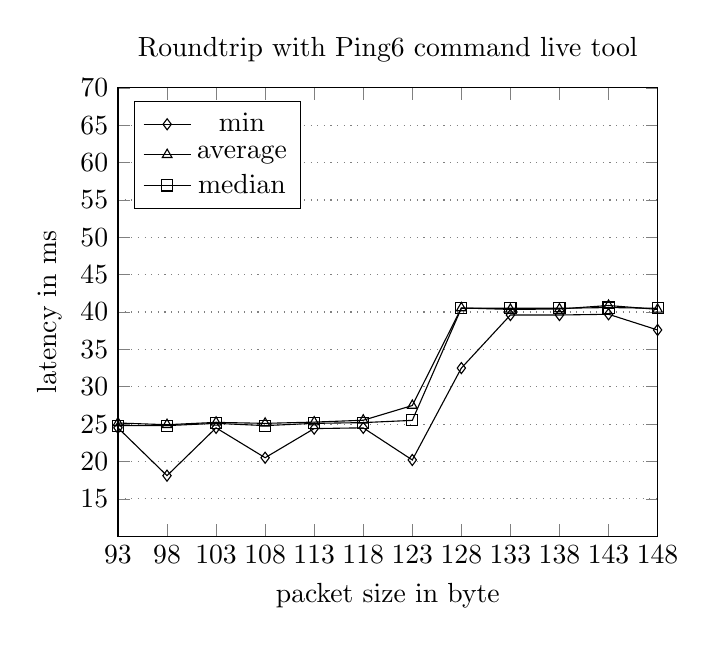
\begin{tikzpicture}
\begin{axis}[
    title={Roundtrip with Ping6 command live tool},
    xlabel={packet size in byte},
    ylabel={latency in ms},
    xmin=93, xmax=148,
    ymin=10, ymax=70,
    xtick={93,98,103,108,113,118,123,128,133,138,143,148,153},
    %xtick={17,22,27,32,42,47,52,57,62,67, 72, 77, 82},
    %ytick={20,40,60,80,100,120,140,160,180,200,220,240},
    ytick={15,20,25,30,35,40,45,50,55,60,65,70},
    legend pos=north west,
    grid style={dotted,gray},
    ymajorgrids=true,
]
\addplot[mark=diamond] coordinates {(93,24.5)(98,18.1)(103,24.5)(108,20.5)(113,24.4)(118,24.5)(123,20.2)(128,32.5)(133,39.6)(138,39.6)(143,39.7)(148,37.6)(153,39.7)};\addlegendentry{min}
\addplot[mark=triangle] coordinates {(93,25.148)(98,24.919)(103,25.232)(108,25.099)(113,25.269)(118,25.515)(123,27.486)(128,40.547)(133,40.349)(138,40.407)(143,40.873)(148,40.353)(153,40.789)};\addlegendentry{average}
\addplot[ mark=square] coordinates {(93,24.8)(98,24.8)(103,25.1)(108,24.8)(113,25.1)(118,25.2)(123,25.5)(128,40.5)(133,40.5)(138,40.5)(143,40.6)(148,40.5)(153,40.5)};\addlegendentry{median}

\end{axis}
\end{tikzpicture}
\caption{Latencies in milliseconds when pinging a sensornode with packet sizes from 93 byte to 148 byte transmitted over the radio. The latencies stays stable at around 27 ms up until 123 byte. After fragmentataion, the latency raise and stay stable at around 43 ms.}
%\caption{The difference between minimum, median and average values is neglectable between packet sizes of 108-123.}
%Latencies in milliseconds when pinging a sensornode with packet sizes from 93 byte to 153 byte transmitted over the radio. The latencies stays stable at around 27 ms up until 123 byte. After fragmentataion, the latency raise and stay stable at around 43 ms.
\label{fig:pingRTT}
\end{figure}

%%%%%%%%%%%%%%%%% WITHOUT DEBUG
\begin{figure}
\centering
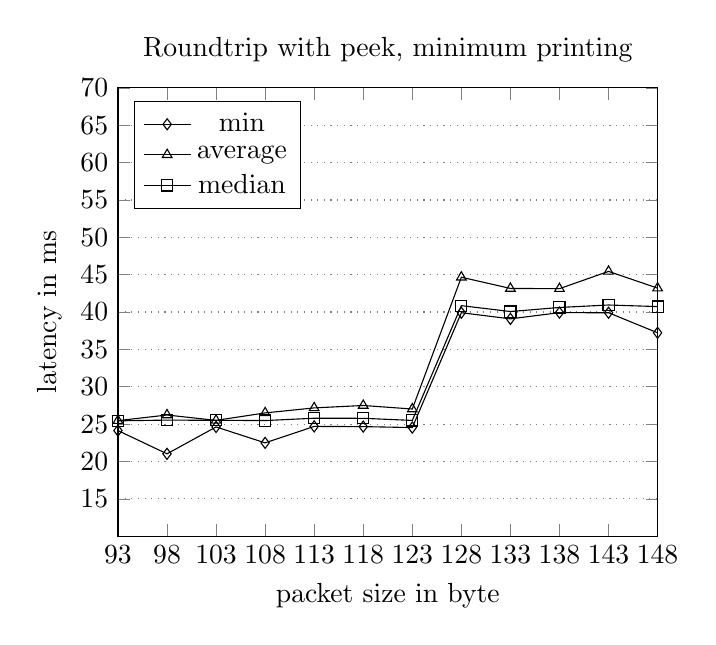
\begin{tikzpicture}
\begin{axis}[
    title={Roundtrip with peek, minimum printing},
    xlabel={packet size in byte},
    ylabel={latency in ms},
    xmin=93, xmax=148,
    ymin=10, ymax=70,
    xtick={93,98,103,108,113,118,123,128,133,138,143,148,153},
    %xtick={17,22,27,32,42,47,52,57,62,67, 72, 77, 82},
    %ytick={20,40,60,80,100,120,140,160,180,200,220,240},
    ytick={15,20,25,30,35,40,45,50,55,60,65,70},
    legend pos=north west,
    grid style={dotted,gray},
    ymajorgrids=true,
]
 
\addplot[ mark=diamond ] coordinates {(93,24.135)(98,21.021)(103,24.62)(108,22.488)(113,24.69)(118,24.663)(123,24.535)(128,39.908)(133,39.0863)(138,39.918)(143,39.904)(148,37.22)};\addlegendentry{min}
\addplot[ mark=triangle ] coordinates {(93,25.46426)(98,26.21715)(103,25.49883)(108,26.49811)(113,27.16887)(118,27.49096)(123,27.01817)(128,44.65865)(133,43.156053)(138,43.12575)(143,45.43817)(148,43.197726)};\addlegendentry{average}
\addplot[ mark=square ] coordinates {(93,25.439)(98,25.535)(103,25.5075)(108,25.4745)(113,25.7845)(118,25.775)(123,25.4915)(128,40.853)(133,40.06595)(138,40.61)(143,40.94)(148,40.7285)};\addlegendentry{median}


\end{axis}
\end{tikzpicture}
\caption{Latencies in milliseconds for peek interest requess of sizes from 93 byte to 148 byte. The latencies stays stable at around 123 ms between 93 byte to 123 byte. After fragmentation, the latency raise and stays stable at around 135 ms instead.}
\label{fig:peekwoutdbRTT}
\end{figure}
%Latencies in milliseconds for peek interest requests of sizes from 93 byte to 153 byte. The latencies stays stable at around 123 ms between 93 byte to 123 byte. After fragmentation, the latency raise and stays stable at around 135 ms instead.
%%%%%%%%%%%%%%%%% WITH DEBUG

\begin{figure}
\centering
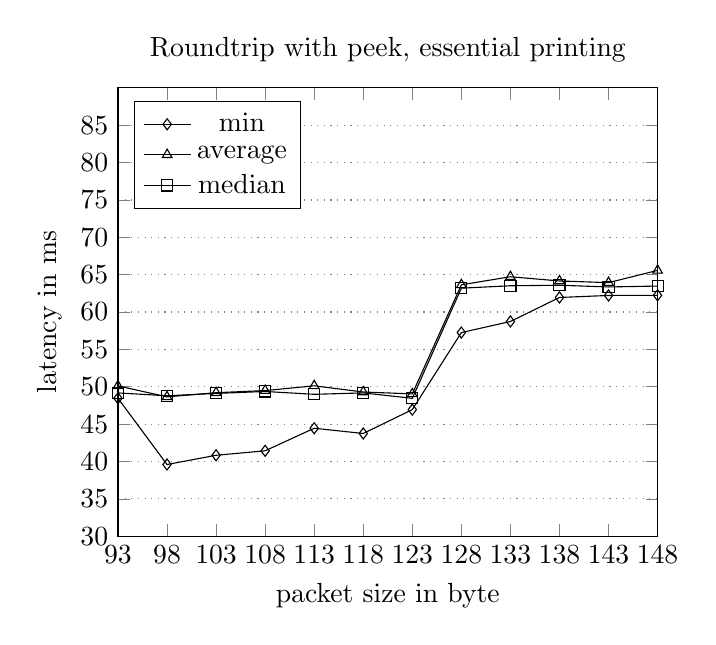
\begin{tikzpicture}
\begin{axis}[
    title={Roundtrip with peek, essential printing},
    xlabel={packet size in byte},
    ylabel={latency in ms},
    xmin=93, xmax=148,
    ymin=30, ymax=90,
    xtick={93,98,103,108,113,118,123,128,133,138,143,148},
    %xtick={17,22,27,32,42,47,52,57,62,67, 72, 77, 82},
    %ytick={20,40,60,80,100,120,140,160,180,200,220,240},
    ytick={15,20,25,30,35,40,45,50,55,60,65,70,75,80,85},
    legend pos=north west,
    grid style={dotted,gray},
    ymajorgrids=true,
]
 
\addplot[ mark=diamond ] coordinates {(93,48.463)(98,39.591)(103,40.828)(108,41.427)(113,44.445)(118,43.744)(123,46.936)(128,57.252)(133,58.734)(138,61.949)(143,62.218)(148,62.236)(153,61.883)};\addlegendentry{min}
\addplot[ mark=triangle ] coordinates {(93,50.11621)(98,48.64623)(103,49.20378)(108,49.48537)(113,50.12659)(118,49.29696)(123,49.0408)(128,63.64151)(133,64.72201)(138,64.15666)(143,63.9334)(148,65.57433)(153,64.98528)};\addlegendentry{average}
\addplot[ mark=square ] coordinates {(93,49.173)(98,48.791)(103,49.108)(108,49.3675)(113,48.987)(118,49.1745)(123,48.451)(128,63.1915)(133,63.516)(138,63.583)(143,63.3555)(148,63.475)(153,63.5055)};\addlegendentry{median}

\end{axis}
\end{tikzpicture}
\caption{Write same as with debugging, or is this graph necessary??}
\label{fig:peekwdbRTT}
\end{figure}



%%%%%%%%%%%%%%%%% PING SICS!!!!
%\begin{figure}
%\centering
%\begin{tikzpicture}
%\begin{axis}[
%    %title={Ping rtt-comparison},
%    xlabel={packet size in byte},
%    ylabel={latency in ms},
%    xmin=93, xmax=148,
%    ymin=10, ymax=70,
%    xtick={93,98,103,108,113,118,123,128,133,138,143,148,153},
%    %xtick={17,22,27,32,42,47,52,57,62,67, 72, 77, 82},
%    %ytick={20,40,60,80,100,120,140,160,180,200,220,240},
%    ytick={15,20,25,30,35,40,45,50,55,60,65,70},
%    legend pos=north west,
%    ymajorgrids=true,
%    grid style={dotted,gray},
%    ymajorgrids=true,
%]
%\addplot[ color=black, ] coordinates {(93,16.7)(98,18.2)(103,19.1)(108,25.6)(113,21.9)(118,20.4)(123,25.8)(128,%35.7)(133,34.0)(138,34.2)(143,37.9)(148,37.1)(153,41.1)};\addlegendentry{min}
%\addplot[ color=blue, ] coordinates {(93,25.653)(98,26.955)(103,26.982)(108,27.331)(113,27.283)(118,26.906)(123%,27.1)(128,42.548)(133,42.245)(138,42.368)(143,42.651)(148,43.245)(153,42.707)};\addlegendentry{average}
%\addplot[ color=red, ] coordinates {(93,26.8)(98,26.9)(103,27.1)(108,27.35)(113,27.3)(118,26.8)(123,27.1)(128,4%2.7)(133,42.5)(138,42.6)(143,42.8)(148,43.0)(153,42.6)};\addlegendentry{median}
%
%\end{axis}
%\end{tikzpicture}
%\caption{SICS BG!!}
%%\caption{The difference between minimum, median and average values is neglectable between packet sizes of %108-123.}
%%Latencies in milliseconds when pinging a sensornode with packet sizes from 93 byte to 153 byte transmitted %over the radio. The latencies stays stable at around 27 ms up until 123 byte. After fragmentataion, the %latency raise and stay stable at around 43 ms.
%\label{fig:scisrtt}
%\end{figure}


\begin{figure}
\centering
\pgfplotstableread[row sep=\\,col sep=&]{
    interval & 17byte & 22byte & 27byte \\
    <20       & 0  & 2  & 0 \\
    20--24    & 0  & 3  & 0  \\
    24--28    & 99 & 95 & 98 \\
    28<       & 1  & 0  & 2 \\
    }\mydata

\begin{tikzpicture}
    \begin{axis}[
            title={Histogram of ping measurements},
            ybar,
            bar width=0.6cm,%<- changed
            %width=\textwidth,
            width=12cm,
            %height=.9\textwidth,
            legend style={at={(0.2,1)},
                anchor=north,legend columns=-1},
            symbolic x coords={<20,20--24,24--28, 28<},
            xtick=data,
            nodes near coords,
            nodes near coords align={vertical},
            ymin=0,ymax=150,
            ytick={0,20,40,60,80,100},
            grid style={dotted,gray},
            ymajorgrids=true,
            height=5cm,
            ylabel={number of roundtrips},
            xlabel={time in ms},
            enlarge x limits={abs=2*\pgfplotbarwidth}
        ]
        \addplot [draw=black,fill=black!60] table[x=interval,y=17byte]{\mydata};
        \addplot [draw=black,fill=black!40] table[x=interval,y=22byte]{\mydata};
        \addplot [draw=black,fill=black!20] table[x=interval,y=27byte]{\mydata};
        \legend{17 , 22 , 27 }
    \end{axis}
\end{tikzpicture}
\caption{Histogram of ping latencies result. A majority of the roundtrips end up in the 24-28 ms span.}
\label{fig:histPing}
\end{figure}

\begin{figure}
\centering
\pgfplotstableread[row sep=\\,col sep=&]{
    interval & 17byte & 22byte & 27byte \\
    <20       & 0  & 0  & 0 \\
    20--24    & 0  & 2  & 0  \\
    24--28    & 100 & 91 & 99 \\
    28<       & 0  & 7  & 1 \\
    }\mydata

\begin{tikzpicture}
    \begin{axis}[
            title={Histogram of peek measurements with minimum printing},
            ybar,
            bar width=0.5cm,%<- changed
            width=12cm,
            %height=.9\textwidth,
            legend style={at={(0.2,1)},
                anchor=north,legend columns=-1},
            symbolic x coords={<20,20--24,24--28, 28<},
            xtick=data,
            nodes near coords,
            nodes near coords align={vertical},
            ymin=0,ymax=150,
            ytick={0,20,40,60,80,100},
            grid style={dotted,gray},
            ymajorgrids=true,
            height=5cm,
            ylabel={number of roundtrips},
            xlabel={time in ms},
            enlarge x limits={abs=2*\pgfplotbarwidth}
        ]
        \addplot [draw=black,fill=black!60] table[x=interval,y=17byte]{\mydata};
        \addplot [draw=black,fill=black!40] table[x=interval,y=22byte]{\mydata};
        \addplot [draw=black,fill=black!20] table[x=interval,y=27byte]{\mydata};
        \legend{17 , 22 , 27 }
    \end{axis}
\end{tikzpicture}
\caption{Histogram of CCN-peek latencies result. Almost all of the roundtrips ended up in the 24-28 ms interval.}
\label{fig:histPeek}
\end{figure}

\newpage
\section{Suitable evaluation test}
\subsection{Purpose}
Follow sequence and periodicity from sensor
The purpose of this experiment is to create a suitable software that follows the periodicity of the data created by a sensor node.

The interval time between the data created by the sensor is known beforehand from the requestor.

\subsection{Delim}
It is not a purpose to find the latest sequence number, this is given at first hand.


\subsection{Method}
Develop software

\begin{itemize}
\item Follow interval on sensor
\item Come to the right sensor
\item First timeout, usage of PIT, one time subscription model
\item After timeout, Algoritm usage to follow/correct

\end{itemize}




\subsection{Result}
Suitable.




Jag har skapat ett program som gör att man kan följa datat som skapas hos en sensor med en konstant interval tid. 

\newpage
\newpage
\section{Discussion}
This section discuss the measurements obtained in Section 4 and 5. %Additionally the methodology used will be discussed.

\subsection{Performance evaluation}
%\begin{itemize}
%\item Clock, jumping result
%\item min values
%\item RTT-values allmänt, diskutera mer utvecklat kring Sparrow. Det tar tid.
%\end{itemize}
The latency performance evaluation was set up to measure hte overhead it takes to compute the CCN communication protocol used as an application for communication between IoT devices. Although the results were impressive overall and gave answers to several questions, they also opened up for further speculations.

Some of the min values that occur are around 40 $\%$ less than the median/average value. At first glance, this was thought to be proof that the general latency time could be lowered, but since there are only a few of these outliers there seem to be other reasons why these lower values occur. They appear more often the smaller the data packet is, which indicates that it is linked with something in the transport layer and how the data is packaged.
%
%One can argue that the round trip times is generally high, with ping6 commands at around 25 ms compared with general speeds of 1-2 ms in a local network. According to the developers of Sparrow, Mats Finne and Joakim Eriksson, it is due to settings in the software that set a delay between each fragment when communicating with the serial-radio. Moreover how the pthread is handling some specific polling function. Due to the fact that it is because of the gateway which affects both cases, it does not effect the performance evaluation in any way.

The round trip time is generally high with ping6 commands at around 25 ms compared with general speeds of 1-2 ms in a local network. One can argue that there are two factors affecting the round trip time. According to the developers of the Sparrow software, Mats Finns and Joakim Eriksson, it is due to settings in the software that set a delay between each fragment when communicating with the serial-radio. Secondly, it depends on the way pthread is handling some specific polling function. Since both of these factors are caused by the same software in the gateway, they do not affect the performance evaluation.

\subsection{Suitability evaluation}
The suitablility evaluation was created to show the feasibility of retrieving data from a sensor that is sequentially produced at a fixed interval with the lowest latency possible. The algorithm developed in this thesis was a first attempt to enable such functionality for ICN in IoT networks.

%\begin{itemize}
%\item Jumping results
%\item Lowering RTTmin
%\item interval, the assumption of same length
%\end{itemize}
The varying round trips shown in the result section have several explanations. The deviation is greater as $\alpha$ grows.
The alternation between values increases as the value on $\alpha$ grows, which in turn impact the \textit{srtt}. 
Deviations can be traced back to values which are for some reason slightly delayed. This is compensated at the next iteration. If it the delay continues, the algortihm overcompensates which results in a devation towards the other side. On the other hand, if the delay becomes stable after the compensation, the variation ends.
One of the reasons why the deviations are approximately the same in size, +- 7-9 ms, is the additional tick it takes to consume an \textit{PIT} entry at the sensor node. This difference is similar to the difference described earlier concerning minimum printing and essential printing in the performance evaluation.

%\begin{itemize}
%\item It handles constant time drift
%\item its not a normal regulator that can change interval
%\item Handles the drift very well.
%\end{itemize}
Currently the algortihm has a small startup curve in order to retreive the \textit{rtt$\_$min}-value before using the PIT of the sensor. After this value is set, there are currently no possibility to recaclulate it or change it later on. This is a known drawback with this algortihm, which could lead to system failure if the \textit{rtt$\_$min} becomes lower than its initiated value. However, problems related to the \textit{rtt$\_$min}, did not occur during the thesis.

A parable with lowering the \textit{rtt$\_$min} is when the interval length on the sensor node is a little shorter in comparison to the interval length set in the algorithm. 
As the results show, the system continued to work for differences up to -2$\%$. Initial tests were done with up to -5$\%$. Then however, the system crashed.

%\begin{itemize}
%\item handle timeouts
%\item Getting wrong sequence, error handling.
%\end{itemize}
The algorithm has limited error correcting capabilities and the results do not show any data on how it handles errors. Two issues that can occur are timeouts and if the algorithm starts to issue \textit{interest} messages with the wrong sequence number. 

It handles timeouts without any greater difficulties for shorter periods of time. Although not shown in the data of the thesis, when a timeout occures, the algorithm continues to successfully send \textit{interest} messages for the next sequence number. This is caused by the serving of the previous correlation factor, so that it is able to keep the ``state'' for some period of time. Since the test was not configured to focus on timeouts specifically, no further investigations have been carried out.

There are more problems to recover from when the sequence number gets unsynced between the producer and the consumer. 
It has not been a task for this thesis to provide any recovery capabilities or the abillity to reconfigure the minimum latency time. Therefore, it has not been tested specifically either, but within the tests carried out by the thesis, some directions and answers have shown how the system handles such errors when they occur.
Depending on how many data entries the producers \textit{cache} can hold, the consumer can be at most the \textit{cache size minus one} sequence numbers after the current data and still be able to retreive the data. 
Another possibility is that the size of the producers \textit{PIT} is large enough to handle several incoming requests and that it is able to hold them for until their data is produced. 




%\subsection{Method Critquie}
%To evaluate the usage of ICN in the IoT domain this thesis has provided an
%
%This thesis has provided an evaluation of the usage of ICN in the IoT domain through an experimental approach. The experiments was done
%To test, 
%The performance was tested under realistic scenarios in a controlled envrionment, as well with the suitablility evaluation.




\newpage

\section{Conclusion}

%\begin{itemize}
%\item Summarize your contributions\\
%The contributions of this report is an algortihm that allows a %consumer to follow the data created, in a periodic interval, on a %sensor node. 
%The data is received in the shortest available time from 
%The time from when the data was created until it has been received %at the 
%
%\item Conclusions from the results
%\item Implications for the future 
%\item Be breif!
%
%\item Its a suitable system. Works flawlessly.
%\end{itemize} 

The aim of this study was to evaluate the useability of ICN in the IoT domain. If it is a suitible candidate that potentially could replace MQTT as an communication paradigm.
The evaluation considered performance measurements of application components, its overall latency and the feasibility of using IoT in the IoT domain.

The performance evaluation showed that the CCN-lite application is successful in deliver a low latency between a sensornode and its gateway. 
When using the CCN peek application to retrieve data from the sensors CCN-lite application, it performs only a few milliseconds slower compared to the ping counterpart.

The optimization of the CCN-lite application code at the sensor shows that part of the long round trip times experienced earlier was due to various debug messages that was printed on the console. Furthermore, the sensor was put into sleep mode of a short period of time for each \textit{interest} message it received. The optimization of the code resulted in around 100 ms faster round trip times compared to before. From round trip times of 130 ms to less than 30 ms.

The suitability evaluation showed that ICN is successful in retreiving low latency values between data creation until it reaches the user. When using of ICNs \textit{PIT} and sending the \textit{interest} messages before the data has been created, ICN can eliminate unnecessary waiting time between data creation and until it is sent. Thereby achiving similar latencies as using MQTT.

The algortihm presented in this thesis is a first attempt to pull data periodically produced at a fixed interval. The algorithm proved to be successful in retreiving data over long periods of time, no timeouts occured during the tests. %In order for it to work properly, it needs a reference time, the length of the interval, 

As the experiment shows presented earlier, the algorithm handles high variations in roundtrip times without any issues. It is because of the logics behind the smoothed round trip time that makes the latency values more or less varying. As $\alpha$ grows, the significance of the smoothed round trip decrease. 

The algorithm handles variances in clock drift to a certain degree. When the data producing interval at the sensor is greater than the consumers, the system stays stable. The length of the \textit{interest} messages timeout, at the consumer, is the only variable that then can cause the algorithm to become unstable. When the data producing interval, at the sensor, is negative compared to the consumer the algortihm handles a limited difference in interval length. The difference between the \textit{rtt$\_$target} and \textit{rtt$\_$min} must be greater than the drift between the consumer interval and the producer, otherwise the system will become unstable.

The conclusions drawn in this thesis is that the communication paradigm ICN provides can be a suitable alternative, in comparision to MQTT, in the IoT domain. A consumer, which was represented as a border gateway, can receive produced data from the producer with a lowest possible latency when it uses the algorithm provided in this thesis. 

%In order for it to work properly, it needs a reference time, length of the interval, 
%It was successful in pulling data even though there was a high $\alpha$,
%Even though the $\alpha$ parameter was changed, which made the round trip times alternate more, the algorithm proved to be stable and successful in retreiving the data.

%Even though round trips alternated, sometimes because of high $\alpha$, the algorithm proved to stay stable and successful in retreiving the data. 
%Even though the round trip times variated, sometimes due to high $\alpha$, the 

%Även om rundtrip tiderna varierade, oftast på grund av ett högt satt alpha, kunde algorithmen parera för detta och leverera datat stabilt till användaren.


%\begin{itemize}
%\item Varfor det fungerar
%\item Fungerar bra for olika deklay pa klockan.
%\end{itemize}
%=======
%\begin{itemize}
%\item Total verdict
%TOTAL verdict.
%The two evaluations combined, have shown that it is feasible to use ICN as a communication paradigm in the IoT domian. 
%\end{itemize}
%
%\begin{itemize}
%\item kort om vad som har gjortst
%\item beskrvi performance evaluation
%\item beskriv feasibile evaluation
%\item beskrvi den mer i detalj.
%\item beskriv helheten att det fungerar bra om man kor det i bode kortare och langre tidsserier.
%\end{itemize}
\newpage
\subsection{Future work}
%To further explore the usage of ICN in IoT networks there are several interesting aspects to consider.
This thesis only showed a subset of the performance and suitability of using ICN in IoT networks. There are several other interesting aspects to consider for future studies. 


\begin{itemize}
\item Scalability
\end{itemize}
%The scalability aspect is 
\begin{itemize}
\item Interval changes on the sensor. Now the drift is constant. Would be interesting to see how it could handle a variated interval.
\end{itemize}





\newpage

%\bibliographystyle{abbrv}
\bibliographystyle{unsrt}
\bibliography{sample}

\end{document}